% Search for all the places that say "PUT SOMETHING HERE".

\documentclass[11pt]{article}
\usepackage{amsmath,textcomp,amssymb,geometry,graphicx,enumerate,tikz}
\usetikzlibrary{arrows}
\geometry{a4paper}
\usepackage{mathtools}
\DeclarePairedDelimiter\ceil{\lceil}{\rceil}
\DeclarePairedDelimiter\floor{\lfloor}{\rfloor}

\def\Name{Nguyet Minh Duong}  % Your name
\def\SID{24444722}  % Your student ID number
\def\Login{N/A} % Your login (your class account, cs170-xy)
\def\Homework{6} % Number of Homework
\def\Session{Spring 2015}


\title{CS170--Fall 2015 --- Homework $\Homework$\textsl{•} Solutions}
\author{\Name, SID \SID}
\markboth{CS170--\Session\  Homework \Homework\ \Name}{CS170--\Session\ Homework \Homework\ \Name}
\pagestyle{myheadings}
\date{}

\newenvironment{qparts}{\begin{enumerate}[{(}a{)}]}{\end{enumerate}}
\def\endproofmark{$\Box$}
\newenvironment{proof}{\par{\bf Proof}:}{\endproofmark\smallskip}

\textheight=9in
\textwidth=6.5in
\topmargin=-.75in
\oddsidemargin=0.25in
\evensidemargin=0.25in


\begin{document}
\maketitle

Collaborators: Henry Kwan \& James Carlson

\section*{1. MST}
\begin{qparts}
\item[1.] Main Idea \\
Run Kruskal's algorithm on the E. This should build us the cheapest roads that connects everywhere. Then we plug in each superhighway one at a time and run Dijkstra on each one to see which one gives a path that uses the superhighway instead. We remember the one that saves us the most cost to create. We build the superhighway (if it satisfy the previous condition) and remove the road (E) with the biggest cost from the start to the end of the superhighway. 
\item[2.] Pseudocode
\begin{verbatim}
Procedure MakeRoads(V, E, S):
  T :=  Kruskal(V, E)
   // Kruskal(V, E) returns a MST using Kruskal's algorithm
 Super := initially null, stores the superhighway that cuts costs
 savedCost := initially null, stores total saved
 T_f := DFS(T, V[1]) // runs DFS on T, and stores its distance from all nodes
   to V[1]
 T_new := initially empty, new graph we return later on
 for each superhighway s in S:
   G := new graph, place s in T
   DFS(G)
   start := left of s where it gets traversed
   end := right of s when it is done traversing   
   distance := T_f(end) - T_f(start) // gives us the distance between the two
   if distance > c(s) and savedCost < distance-c(s):
     Super = s
     savedCost = distance - c(s)
     R := biggest road from start to end
     T_new := T removed R added Super
 if T_new is null:
   T_new = T
 return T_new
  
\end{verbatim}
\item[3.] Proof of Correctness \\
Kruskal's algorithm will give us the best road path to connect all of the cities together by its definition. And by manually plugging in all of the of the s, and comparing its distance with the original takes to get to the begining of the highway to the end, will allow us to be able to tell whether or not the manual way takes longer. If it does, how much do we save from it -- how much we save must be greater than all other highways savings. If it is, we change our highway saving, and the superhighway we want to build. Then we run through the path to see which road took up the most cost and remove it. This works because we are manually forcing it to run a specific way. 
 
\item[4.] Running Time Analysis \\
$O(S(E+V))$ \\

Kruskal's take $O(ElogE)$, DFS takes $O(E+V)$. We only did Kruskal's once, but we had to do run DFS S-times, which is $O(S(E+V))$. Removal and adding the lines in takes $O(S)$ times, which is significantly smaller than the previous. $O(ElogE)$ is also significantly smaller as well. Therefore our algorithm's longest run time is due to our search on which path is the best. 
The reason for 
\end{qparts}
\newpage
\section*{2. Sorted Sequences}
\begin{qparts}
\item[1.] Main Idea \\
We sort all the lines we have from smallest to biggest. Then in the first instance, right after sorting all the hobbits (bunnies???), we take the first two lines and merge them. Thisultimately be the least amount of time it takes to merge any two lines because it has the least amount of hobbits in both, therefore it require the least amount of merging. We move the newly formed merge line somewhere else. Now we compare the possible merges, which are the first two lines in each list of lines. Compare these (at most) four lines in how long they are. Choose the two that are the shortest, merge, and put it in the back of the second line. Repeat until there is only one line left -- meaning if the first list have no more lines, create a new list and repeat the process. 
\item[2.] Pseduocode
\begin{verbatim}
Procedure SortHobbits(list Lines):
  L2 := a new empty list of lines
  sortBySize(Lines) // sorts Lines by size of each line, shortest to longest
  state := tells us which list newly formed lines should go to, initially null
    
  while true:
    if isEmpty(Lines) or isEmpty(L2): 
      if size(Lines) = 1:
        return Lines.pop() // returns & removes the first value in list
      else if size(L2) = 1: 
        return L2.pop()
      else if isEmpty(Lines):
        L = L2.pop() + L2.pop() // assume + sign merges the lines
        Lines.push(L)
          // push(L) puts L at the end of the list
        state := Lines
      else:
        L = Lines.pop() + Lines.pop()
        L2.push(L)
        state := L2
    else:
      V1, V2 = first two values in Lines, if possible --
        if not, return infinity. Does not remove from Lines
      V3, V4, first two values in L2, if possible --
        if not, return infinity. Does not remove from L2
      S1, S2 = two shortest lines from {V1, V2, V3, V4} 
      remove S1 from appropriate list
      remove S2 from appropriate list
      state.push(S1 + S2)
\end{verbatim}
\item[3.] Proof of Correctness \\
First, it is key to understand that long lines of hobbits will take a very long time, so we want to do it the least as possible. Meaning, we should always merge the shorter lines before moving onto the lines that are longer. Therefore it is in our best interest to always merge the shorter lines against each other. That's why we start off by sorting all of the lines from shortest to longest, and merging the first one. We move it to a second list so that we do not have to reorder the lists, which would cause the program to take exponential time of figuring it out. \\

Our second list is ordered and so is our first. The second list is ordered because we are always adding the merged lines at the end. The merged lines adding to the second list will always be the longest or equal to the one to the left of it because the previous is made of two lines shorter than the two lines we are merging at the moment. We know this because we choose the two smallest lines first. The only way for the next merged line value to be smaller is if you choose two values such that they are equal or smaller than what we used to create the previous in the second list. This is not possible because as mentioned, we have sorted the list. Therefore the creation of the second list is also sorted. \\

Since we choose the shortest lines first, we fulfilled our initial key understanding. All the shorter lines are merged first before moving onto the bigger ones. We should always merge lines that are short as this will take less time to merge since it's a lower value. 
\item[4.] Running Time Analysis \\
$O(nlogn)$ where n is the number of lines we are initially given. \\
We start by sorting the lines by mergesort, which has the run time of $O(nlogn)$. Then we look at the four different lines -- the first two in the first list, and the first two in the second list. We then find the two smallest lines within this subset. The time it takes to figure out the two shortest lines is at most $O(8)$, where we mergesort is ($4log4 = 8$) and then we combine the two shortest lines into one. This means that we will have to do approximately $8logn$ comparison because we are comparing every 2 values. So if we combine the run times together, our $O(nlogn)$ dominates the constants and $O(logn)$. Hence our answer. 
\end{qparts}

\newpage
\section*{3. Timesheet}
First, it is key to note that the bonuses $V$ does not matter in this case because it remainds static. We get all of the bonuses in the end ($V_{total} = \sum_{i=1}^{N} V_i$), and we subtract the total amount of penalty from $V_{total}$. Therefore our problem here is to find the order in which the penalty is the least. \\

To minimize the penalty, we need to choose the job that will grow greatest in cost of penalty over time and get it out of the way first. And repeat this until there are no more jobs left to do. We figure this out by taking the ratio between the penalty cost and days required to complete the job ($\frac{P_i}{R_i}$). The job that is most pessimal is equivalent to the one with the biggest penalty cost to days ratio. \\


The reason that the ratios determine which job is the most pessimal is because we can visualize this problem as a graph, where the x-axis is time, and y-axis is penalty. Our goal in this graph is to place the blocks of penalty in such a way that it minimizes the height of the graph. The ratio, now slope, will allow us to visualize how fast it grows over time. By using calculus, we know that the area under the line created by the slope with y-intersection as 0 is the total amount of penalty we have accumilated. It is key to know that we want to start one job right after the next because we don't want to go over by a day because this means we are losing money for no reason. So we know that the total amount of days we need to finish the job is $T = \sum_{i=1}^{N} R_i$. \\

Now if we plug in the slope into the equation of a line, and have it end at T, we see that the one with the biggest slope will get the penalty -- meaning it will end the highest. Therefore we want to get it out of the way first. The we keep going and see which ratio gets the highest y-value at T, and do that job right away. This way, we minimize the amount of penalty we have to get. Therefore it is the most efficient. 
\newpage
\section*{4. 2SAT}
\begin{qparts}
\item[1.] Main Idea \\
Given the clauses, we will create a tree based on the following idea: create a directed edge from the first literal to the negated second literal, then vice versa. Place these nodes and edges in a graph G. While make these directed edges per clause, we store them in a list of pairs called P. We insert them in as paired up values. Then we start by looking at the node with the biggest number outgoing edges. Make the literal, call it L, in that true. Remove edges that are L's pairs (L to whatever node). Repeat the algorithm until we have marked all the nodes with outgoing edges. 
\item[2.] Pseudocode
\begin{verbatim}
// Clauses is an object that has literal variables
// left and right 
// Literals can be asked if they are the the same literal (object)
Procedure Satisfiable(Clauses C[]):
  G := an empty graph
  E := list of edges
    // can ask for its paired edge
  V := list of nodes
    // nodes can be asked whether or not it is True or False
    // may be null if unknown
    // can be asked for its negated node pair and will return
    // the opposite of its True/False value
  for all clause in C:
    if leftLiteral(clause) is the same as rightLiteral(clause):
      L = leftLiteral(clause)
      L_node := node with L value
      Input L_node into list V
      if isNegated(L):
        value(L_node) = False
      else:
        value(L_node) = True
      Ln_node := node with negated L value
      X := edge from L_node to Ln_node in G
      input edge into E
    else:
      L = leftLiteral(clause)
      R = rightLiteral(clause)
      R_node := node with R value
      L_node := node with L value
      Rn_node := node with negated R value
      Ln_node := node with negated L value
      X := edge from L_node to Rn_node in G
      Y := edge from R_node to Ln_node in G
      input edges into E
      Pair(X, Y)
  while nodes are not all marked:
  	N := node with most outgoing edge,
  	  if there are more than one, pick one randomly
  	if value(N) is null or True:
  	  value(N) = True
  	  mark(N)
  	  for all edge X outgoing from N:
  	    remove edge PairOf(X) // removes the edge that is paired with X
      Neg := negated node of N
      for all edge X outgoing from Neg:
        remove edge X
    if value(N) is False:
      for all edge X outgoing from N:
        remove edge X
      Neg := negated node of N
      for all edge X outgoing from Neg:
        remove edge PairOf(X)
  if NumberOfEdges(E) < NumberOfClauses(C):
    return "Not Possible"
  else:
    return "Possible!"

\end{verbatim}
\item[3.] Proof of Correctness \\
For a single clause, there is two ways for it to be true and it is if its left literal ($L_i$) is true, and its right literal is false ($L_j$) or $L_j$ is true and $L_i$ is false. This is trivial. What this also means is that if we already proved one statement is true, we do not need to prove the other one. Hence why we remove its paired edge because in our algorithm we decided to show which one is true by the outgoing directed edge. We choose the nodes with the highest of outgoing edges because it will allow more clauses to be true, since that is what our outgoing edge indicates. We mark the node as visited so we know that we have already assesed its value. \\

But if that node is True, its negated node must be False. What this means is that the outgoing edges is no longer true because of how we have defined the edges to mean (stating that the combination is True, which is not true because its negated value is now False). \\ 

Then we continue on, making sure we have saved its True or False states. In theory, we should never visit a node that is True, but if we do, we implement the save thing. In addition, when we visit a node that is False, it should have zero outgoing edge and not do anything because by it having a value, we have already went ahead and do what it is supposed to be done. But the pseudocode is included for this case such that we just do the opposite of the True one. 


\item[4.] Running Time Analysis \\
$O(N)$ where N is the number of literals. \\

We run through the clauses, and read the literals and create its appropriate nodes and its negation. This is $O(2N)$ because we have to create the paired negations of the nodes, along with the appropriate edges. We create $2N$ edges, therefore this takes $O(2N)$ because for every clause we create two directed components. Then in our algorithm, we look through every single node. This is $O(2N)$ because we created its negations as well. Within this, we remove edges appropriate with the algorithm, which should be constant time. Note that our number of edges is $O(2N)$ because for every clause, we created two directed edges. At the end, we check the number of edges we have, which is constant time, against how many clauses we have. So in total, it is $O(2N) + O(2N) + O(2N) + O(2N) \rightarrow O(N)$ because we don't care about the constant values in bigO.
\end{qparts}

\newpage
\section*{5. Right or Wrong}
\begin{qparts}
\item True. Proof by contradiction. \\
Assume that using Kruskals algorithm, we create a subgraph G with \textit{k} edges such that there exists another subgraph G' such that it is lighter with the same amount of edges. This means that there is a lighter edge that can be substituted for an edge in G. However this would contradict with Kruskal's algorithm because it has already sorted the list of edges by its edge weight, and will pick the lightest valid edge first. Therefore if there exists a lighter edge to substitute in G, this edge will probably create a cycle in the graph, which will not create a minimum spanning tree. 

\item False. Counterexample:  For $K = 2$, it will not satisfy the statement in the problem. \\
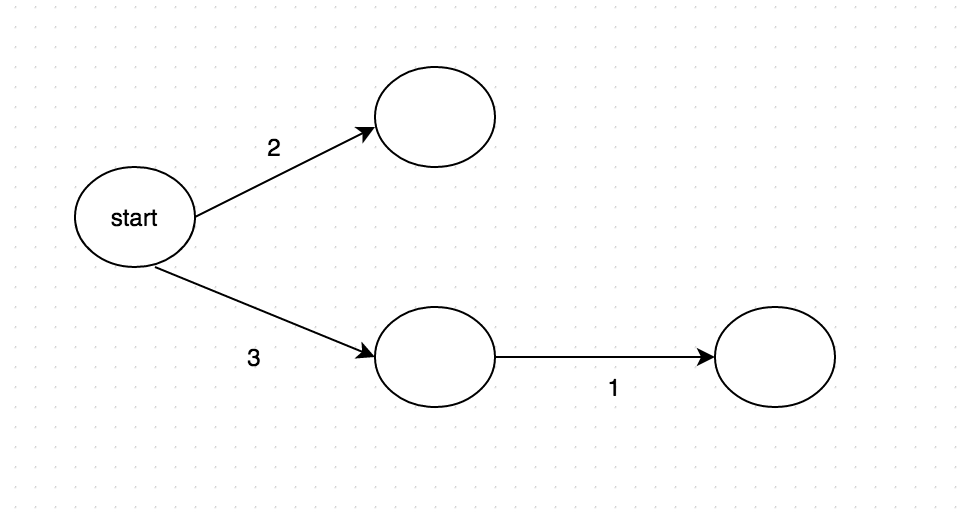
\includegraphics[scale=0.7]{counter} \\
The reason for this is because if we follow Prim's Algorithm, we would visit the node that is connected by the edge of length 2, and then the node by the edge of length 3, giving us a total of 5. However there exists another pattern we could have gone, which is to the node of edge of length 3, then to the node by the edge of length 1, giving us a total of 4. 


\end{qparts}

\end{document}
